% ============================================================
% Modul 02: Deep Learning Fundamentals
% Custom NVIDIA Dark Beamer Theme
% Compiler: xelatex
% ============================================================
\documentclass[aspectratio=169,t]{beamer}

% ---- Fonts (xelatex) ----------------------------------------
\usepackage{fontspec}
\usepackage[sfdefault]{FiraSans}

% ---- Bahasa (pola pemenggalan Indonesia) --------------------
\usepackage[indonesian]{babel}

% Kata Inggris yang dipenggal salah oleh pola Indonesia
\hyphenation{train vari-ance scal-ing de-ci-sion boost-ing gra-di-ent
  drop-out soft-max learn-ing back-prop op-ti-mi-zer va-nish-ing
  po-oling con-vo-lu-tion em-bed-ding}

% ---- Core packages ------------------------------------------
\usepackage{graphicx}
\usepackage{tikz}
\usetikzlibrary{positioning, shapes.geometric, arrows.meta, calc}
\usepackage{pgfplots}
\pgfplotsset{compat=1.18}
\usepackage{amsmath}
\usepackage{booktabs}
\usepackage{colortbl}
\usepackage{xcolor}
\usepackage{listings}

% ============================================================
% COLOR PALETTE
% ============================================================
\definecolor{nvbg}{HTML}{1A1A2E}        % dark navy background
\definecolor{nvdark}{HTML}{1A1A2E}     % alias for nvbg
\definecolor{nvcard}{HTML}{2D2D44}      % card / box background
\definecolor{nvgreen}{HTML}{76B900}     % NVIDIA green (primary accent)
\definecolor{nvlightgreen}{HTML}{A3D944}% secondary accent
\definecolor{nvwhite}{HTML}{FFFFFF}
\definecolor{nvgray}{HTML}{AAAACC}      % muted text
\definecolor{nvdarkcard}{HTML}{23233A}  % slightly darker card
\definecolor{nvred}{HTML}{EF5350}       % accent red
\definecolor{nvorange}{HTML}{FF6F00}    % accent orange

% ============================================================
% LISTINGS STYLE
% ============================================================
\lstset{
  backgroundcolor=\color{nvcard},
  basicstyle=\ttfamily\small\color{nvwhite},
  keywordstyle=\color{nvgreen}\bfseries,
  stringstyle=\color{nvlightgreen},
  commentstyle=\color{nvgray}\itshape,
  numberstyle=\tiny\color{nvgray},
  numbers=left,
  numbersep=6pt,
  frame=none,
  breaklines=true,
  showstringspaces=false,
  tabsize=2,
  xleftmargin=8pt,
  xrightmargin=4pt,
}

% ============================================================
% BEAMER THEME — NVIDIA DARK
% ============================================================
\usetheme{default}
\usecolortheme{default}
\setbeamercolor{normal text}{fg=nvwhite, bg=nvbg}
\setbeamercolor{background canvas}{bg=nvbg}
\setbeamercolor{frametitle}{fg=nvwhite, bg=nvbg}
\setbeamercolor{title}{fg=nvgreen}
\setbeamercolor{subtitle}{fg=nvwhite}
\setbeamercolor{author}{fg=nvgray}
\setbeamercolor{date}{fg=nvgray}
\setbeamercolor{item}{fg=nvgreen}
\setbeamercolor{subitem}{fg=nvlightgreen}
\setbeamercolor{subsubitem}{fg=nvgray}
\setbeamercolor{block title}{fg=nvwhite, bg=nvcard}
\setbeamercolor{block body}{fg=nvwhite, bg=nvdarkcard}
\setbeamercolor{alerted text}{fg=nvgreen}
\setbeamercolor{structure}{fg=nvgreen}
\setbeamercolor{footline}{fg=nvgray, bg=nvbg}
\setbeamercolor{section in toc}{fg=nvwhite}

% Remove navigation symbols
\setbeamertemplate{navigation symbols}{}

% ---- Frame title with green underline -----------------------
\setbeamertemplate{frametitle}{%
  \vspace{0.3em}%
  \begin{beamercolorbox}[wd=\paperwidth, leftskip=0.5cm]{frametitle}%
    {\large\bfseries\insertframetitle}%
    \ifx\insertframesubtitle\@empty\else
      \\[0.1em]{\small\color{nvgray}\insertframesubtitle}%
    \fi
  \end{beamercolorbox}%
  \begin{tikzpicture}[overlay, remember picture]
    \draw[nvgreen, line width=1.5pt]
      ([xshift=0.5cm, yshift=-0.1cm]current page.north west)
      -- ([xshift=-0.5cm, yshift=-0.1cm]current page.north east);
  \end{tikzpicture}%
  \vspace{-0.3em}%
}

% ---- Footer -------------------------------------------------
\setbeamertemplate{footline}{%
  \begin{beamercolorbox}[wd=\paperwidth, ht=2.2ex, dp=1.2ex]{footline}%
    \hspace{0.6cm}%
    {\footnotesize\color{nvgray}Deep Learning Fundamentals}%
    \hfill%
    {\footnotesize\color{nvgray}\insertframenumber\,/\,\inserttotalframenumber}%
    \hspace{0.6cm}%
  \end{beamercolorbox}%
}

% Remove headline
\setbeamertemplate{headline}{}

% Itemize bullets
\setbeamertemplate{itemize item}{\color{nvgreen}\rule[0.3ex]{0.55em}{0.55em}}
\setbeamertemplate{itemize subitem}{\color{nvlightgreen}\small$\blacktriangleright$}

% ============================================================
% CUSTOM COMMANDS
% ============================================================

% \acttitle{Act N}{Title}{Subtitle/question}
\newcommand{\acttitle}[3]{%
  \begin{frame}[plain]
    \begin{tikzpicture}[remember picture, overlay]
      % Full dark background
      \fill[nvbg] (current page.south west) rectangle (current page.north east);
      % Subtle horizontal accent bar
      \fill[nvgreen] ([yshift=-2pt]current page.north west)
        rectangle ([yshift=-5pt]current page.north east);
      % Act label (top-left, small)
      \node[anchor=north west, xshift=1.2cm, yshift=-1.0cm,
            font=\large\bfseries, text=nvgreen] at (current page.north west) {#1};
      % Main title (center, large, NVIDIA green)
      \node[anchor=center, yshift=0.5cm,
            font=\fontsize{32}{36}\selectfont\bfseries, text=nvgreen]
            at (current page.center) {#2};
      % Subtitle / question (center, below, white)
      \node[anchor=center, yshift=-1.0cm,
            font=\large, text=nvwhite]
            at (current page.center) {\textit{#3}};
      % Bottom accent line
      \draw[nvcard, line width=2pt]
        ([xshift=2cm, yshift=2.0cm]current page.south west)
        -- ([xshift=-2cm, yshift=2.0cm]current page.south east);
    \end{tikzpicture}
  \end{frame}%
}

% Colored info box
\newcommand{\nvbox}[2]{%
  \begin{tikzpicture}
    \node[fill=nvcard, rounded corners=4pt, inner sep=8pt,
          text width=\linewidth-16pt, text=nvwhite]
      {\textbf{\color{nvgreen}#1}\\\medskip#2};
  \end{tikzpicture}%
}

% \intuisi{Judul} -> frametitle "Judul" + tag kecil "Intuisi" di kanan atas
\newcommand{\intuisi}[1]{%
  \frametitle{\makebox[\dimexpr\paperwidth-1.7cm\relax][l]{%
    #1\hfill{\small\color{nvlightgreen}Intuisi}}}}

% \jebakan{teks} -> kotak oranye
\newcommand{\jebakan}[1]{%
  \begin{tikzpicture}
    \node[fill=nvorange!25!nvbg, draw=nvorange, rounded corners=4pt, inner sep=7pt,
          text width=\linewidth-16pt, text=nvwhite]
      {\textbf{\color{nvorange}Jebakan:} #1};
  \end{tikzpicture}%
}

% \kapan{cocok}{kurang cocok} -> dua kolom hijau/merah
\newcommand{\kapan}[2]{%
  \begin{columns}[T]
    \begin{column}{0.48\textwidth}
      \textbf{\color{nvgreen}Cocok kalau}
      \begin{itemize}#1\end{itemize}
    \end{column}
    \begin{column}{0.48\textwidth}
      \textbf{\color{nvred}Kurang cocok kalau}
      \begin{itemize}#2\end{itemize}
    \end{column}
  \end{columns}%
}

% ============================================================
% TITLE INFO
% ============================================================
\title{\color{nvgreen}Deep Learning Fundamentals}
\subtitle{Navasena Gen-ML Course}
\author{Navasena AI}
\date{}

% ============================================================
% DOCUMENT
% ============================================================
\begin{document}

% ==========================================================
% ACT 0
% ==========================================================

% ----------------------------------------------------------
% FRAME 1 — Judul
% ----------------------------------------------------------
\begin{frame}[plain]
  \begin{tikzpicture}[remember picture, overlay]
    \fill[nvbg] (current page.south west) rectangle (current page.north east);
    \fill[nvgreen] ([yshift=-3pt]current page.north west)
      rectangle ([yshift=-7pt]current page.north east);
    \fill[nvgreen!30] (current page.south west)
      rectangle ([xshift=6pt]current page.north west);
    \node[anchor=center, yshift=1.6cm,
          font=\fontsize{28}{32}\selectfont\bfseries, text=nvgreen]
          at (current page.center) {Deep Learning Fundamentals};
    \node[anchor=center, yshift=0.5cm, font=\large, text=nvwhite]
          at (current page.center)
          {Hari 2 \textperiodcentered{} Navasena Gen-ML Course \textperiodcentered{} Batch 6};
    \draw[nvgreen, line width=1pt]
      ([xshift=-5cm]current page.center) -- ([xshift=5cm]current page.center);
    \node[anchor=center, yshift=-0.6cm, font=\normalsize, text=nvgray]
          at (current page.center)
          {6 notebook \textperiodcentered{} TensorFlow dan Keras \textperiodcentered{} Google Colab};
    \node[anchor=center, yshift=-1.5cm, font=\small, text=nvgray]
          at (current page.center) {Navasena AI};
  \end{tikzpicture}
\end{frame}

% ----------------------------------------------------------
% FRAME 2 — Peta hari 2
% ----------------------------------------------------------
\begin{frame}{Peta hari 2}
  \vspace{0.2em}
  \begin{center}
  \begin{tikzpicture}[
    card/.style={fill=nvcard, rounded corners=4pt, inner sep=7pt, text width=3.15cm,
                 text=nvwhite, font=\scriptsize, anchor=north west, align=left}]
    \node[card] at (0,0)
      {{\bfseries\color{nvgreen}Dasar belajar}\\[2pt]
       nb01 Neural network pertama (Fashion-MNIST)};
    \node[card] at (4.15,0)
      {{\bfseries\color{nvlightgreen}Aktivasi}\\[2pt]
       nb02 Fungsi aktivasi dan optimizer};
    \node[card] at (8.3,0)
      {{\bfseries\color{nvorange}Gambar}\\[2pt]
       nb03 CNN dan transfer learning (CIFAR-10)};
    \node[card] at (0,-2.7)
      {{\bfseries\color{nvgreen}Urutan}\\[2pt]
       nb04 RNN dan LSTM};
    \node[card] at (4.15,-2.7)
      {{\bfseries\color{nvlightgreen}GPU}\\[2pt]
       nb05 Mixed precision, ONNX, TensorRT};
    \node[card] at (8.3,-2.7)
      {{\bfseries\color{nvorange}Generatif}\\[2pt]
       nb06 Autoencoder, GAN, diffusion};
  \end{tikzpicture}
  \end{center}
  \vspace{0.4em}
  {\footnotesize\color{nvgray}Dua act pertama membahas cara satu neural network belajar. Sisanya
  memakai dasar itu untuk gambar, urutan, GPU, dan model generatif.}
\end{frame}

% ----------------------------------------------------------
% FRAME 3 — Jembatan dari hari 1
% ----------------------------------------------------------
\begin{frame}{Dari hari 1 ke hari 2}
  \vspace{0.1em}
  \begin{columns}[T]
    \begin{column}{0.48\textwidth}
      \textbf{\color{nvlightgreen}ML klasik (hari 1)}
      \vspace{0.4em}
      \begin{itemize}\setlength\itemsep{0.42em}
        \item Feature dipilih dan dirancang manusia: kolom umur, gaji, durasi
        \item Data tabular, satu baris satu contoh
        \item Modelnya kecil, koefisiennya bisa dibaca satu per satu
      \end{itemize}
    \end{column}
    \begin{column}{0.48\textwidth}
      \textbf{\color{nvgreen}Deep learning (hari 2)}
      \vspace{0.4em}
      \begin{itemize}\setlength\itemsep{0.42em}
        \item Feature dipelajari dari data mentah: pixel, urutan kata
        \item Gambar, teks, dan sinyal berurutan
        \item Modelnya berlapis, jumlah parameternya ratusan ribu ke atas
      \end{itemize}
    \end{column}
  \end{columns}
  \vspace{0.5em}
  \nvbox{Yang tidak berubah}{Alur kerjanya sama seperti hari 1: pisahkan data train,
  validation, dan test; bandingkan dengan baseline; pilih model di data validation.
  Yang berubah adalah bentuk modelnya dan dari mana featurenya datang.}
\end{frame}

% ==========================================================
% ACT 1
% ==========================================================
\acttitle{Act 1}{\fontsize{26}{30}\selectfont\bfseries Bagaimana neural network belajar?}{Satu angka kesalahan, lalu diperbaiki sedikit demi sedikit}

% ----------------------------------------------------------
% FRAME 5 — Intuisi: satu neuron
% ----------------------------------------------------------
\begin{frame}
  \intuisi{Satu neuron: jumlah berbobot, lalu diputuskan}
  \vspace{0.2em}
  \begin{center}
  \begin{tikzpicture}[scale=0.95, font=\scriptsize,
    inp/.style={circle, fill=nvcard, text=nvwhite, minimum size=0.62cm, inner sep=0pt},
    box/.style={fill=nvcard, rounded corners=3pt, text=nvwhite, inner sep=5pt}]
    \node[inp] (x1) at (0,1.5) {$x_1$};
    \node[inp] (x2) at (0,0.6) {$x_2$};
    \node[inp] (x3) at (0,-0.3) {$x_3$};
    \node[circle, draw=nvgreen, line width=1pt, fill=nvbg, text=nvwhite,
          minimum size=1.0cm] (s) at (3.6,0.6) {$\Sigma$};
    \node[box] (act) at (6.4,0.6) {aktivasi};
    \node[text=nvgray] (b) at (3.6,-1.5) {bias $b$};
    \draw[nvgreen, -{Stealth[length=4pt]}] (x1) -- node[above, sloped, text=nvlightgreen, font=\tiny] {$w_1$} (s);
    \draw[nvgreen, -{Stealth[length=4pt]}] (x2) -- node[above, sloped, text=nvlightgreen, font=\tiny] {$w_2$} (s);
    \draw[nvgreen, -{Stealth[length=4pt]}] (x3) -- node[below, sloped, text=nvlightgreen, font=\tiny] {$w_3$} (s);
    \draw[nvgray, -{Stealth[length=4pt]}] (b) -- (s);
    \draw[nvgreen, -{Stealth[length=4pt]}] (s) -- (act);
    \draw[nvgreen, -{Stealth[length=4pt]}] (act) -- ++(2.1,0)
      node[right, text=nvwhite] {keluaran};
    \node[text=nvgray, font=\tiny, anchor=east] at (2.55,-1.5) {$w_1x_1+w_2x_2+w_3x_3+b$};
  \end{tikzpicture}
  \end{center}
  \vspace{0.2em}
  \nvbox{Intinya}{Bobot adalah takaran: seberapa besar tiap masukan ikut dihitung. Bias
  menggeser hasilnya. Aktivasi menentukan bentuk keluaran neuron.}
\end{frame}

% ----------------------------------------------------------
% FRAME 6 — Layer dan arsitektur
% ----------------------------------------------------------
\begin{frame}{Dari satu neuron ke satu arsitektur}
  \vspace{0.1em}
  \begin{center}
  \begin{tikzpicture}[scale=0.92, font=\tiny,
    n/.style={circle, fill=nvlightgreen, minimum size=0.24cm, inner sep=0pt}]
    \foreach \y in {0,1,2,3} { \node[n] (a\y) at (0,\y*0.72) {}; }
    \foreach \y in {0,1,2,3} { \node[n] (b\y) at (3.0,\y*0.72) {}; }
    \foreach \y in {0,1,2}   { \node[n] (c\y) at (6.0,\y*0.72+0.36) {}; }
    \foreach \y in {0,1,2}   { \node[n] (d\y) at (9.0,\y*0.72+0.36) {}; }
    \foreach \i in {0,1,2,3} \foreach \j in {0,1,2,3}
      \draw[nvcard, line width=0.35pt] (a\i) -- (b\j);
    \foreach \i in {0,1,2,3} \foreach \j in {0,1,2}
      \draw[nvcard, line width=0.35pt] (b\i) -- (c\j);
    \foreach \i in {0,1,2} \foreach \j in {0,1,2}
      \draw[nvcard, line width=0.35pt] (c\i) -- (d\j);
    \node[text=nvwhite, anchor=north, align=center] at (0,-0.45)
      {\textbf{784}\\ pixel\\ (Flatten)};
    \node[text=nvwhite, anchor=north, align=center] at (3.0,-0.45)
      {\textbf{128}\\ Dense\\ ReLU};
    \node[text=nvwhite, anchor=north, align=center] at (6.0,-0.45)
      {\textbf{64}\\ Dense\\ ReLU};
    \node[text=nvwhite, anchor=north, align=center] at (9.0,-0.45)
      {\textbf{10}\\ Dense\\ softmax};
    \node[text=nvgray, anchor=west] at (10.1,1.1) {tiap neuron};
    \node[text=nvgray, anchor=west] at (10.1,0.75) {terhubung ke};
    \node[text=nvgray, anchor=west] at (10.1,0.4) {semua neuron};
    \node[text=nvgray, anchor=west] at (10.1,0.05) {layer sebelumnya};
  \end{tikzpicture}
  \end{center}
  \vspace{0.4em}
  \begin{itemize}\setlength\itemsep{0.28em}
    \item Flatten menggelar gambar 28$\times$28 menjadi satu baris berisi 784 angka.
    \item Dua hidden layer menyusun feature: layer berikutnya bekerja di atas keluaran
          layer sebelumnya.
    \item Output layer punya 10 neuron, satu untuk tiap kategori pakaian.
  \end{itemize}
\end{frame}

% ----------------------------------------------------------
% FRAME 7 — Bobot dan bias
% ----------------------------------------------------------
\begin{frame}{Yang berubah saat model belajar}
  \vspace{0.6em}
  \begin{center}
  {\small\renewcommand{\arraystretch}{1.3}
  \begin{tabular}{lrrr}
    \toprule
    \rowcolor{nvcard}\color{nvgreen}\textbf{Layer} &
    \color{nvgreen}\textbf{Bobot} &
    \color{nvgreen}\textbf{Bias} &
    \color{nvgreen}\textbf{Parameter} \\
    \midrule
    Dense 128 (ReLU)    & $784\times128$ & 128 & 100.480 \\
    Dense 64 (ReLU)     & $128\times64$  & 64  & 8.256 \\
    Dense 10 (softmax)  & $64\times10$   & 10  & 650 \\
    \midrule
    \textbf{Total}      &                &     & \textbf{109.386} \\
    \bottomrule
  \end{tabular}}
  \end{center}
  \vspace{0.7em}
  \begin{itemize}\setlength\itemsep{0.3em}
    \item Seratus ribu angka ini dimulai dari nilai acak, lalu diperbaiki selama training.
    \item Jumlah layer, jumlah neuron, dan learning rate kamu tentukan sebelum training;
          ketiganya bukan hasil training.
  \end{itemize}
\end{frame}

% ----------------------------------------------------------
% FRAME 8 — Loss
% ----------------------------------------------------------
\begin{frame}{Loss: satu angka yang mengukur seberapa salah}
  \vspace{0.5em}
  \begin{center}
    \color{nvlightgreen}$\displaystyle \text{loss satu contoh} = -\log\left(p_{\text{kelas benar}}\right)$
  \end{center}
  \vspace{0.5em}
  \begin{itemize}\setlength\itemsep{0.42em}
    \item Model mengeluarkan satu probabilitas untuk tiap kelas. Loss hanya melihat
          probabilitas yang diberikan ke kelas yang benar.
    \item Probabilitas 0,85 untuk kelas yang benar memberi loss kecil; 0,05 memberi loss besar.
    \item Loss seluruh batch adalah rata-rata loss tiap contohnya. Angka inilah yang
          diperkecil saat training.
  \end{itemize}
  \vspace{0.5em}
  {\footnotesize\color{nvgray}Namanya di Keras: \texttt{sparse\_categorical\_crossentropy}.
  Accuracy dilaporkan untuk kita baca; loss yang dipakai model untuk memperbaiki diri.}
\end{frame}

% ----------------------------------------------------------
% FRAME 9 — Intuisi: gradient descent
% ----------------------------------------------------------
\begin{frame}
  \intuisi{Gradient descent: menuruni bukit dalam kabut}
  \vspace{0.1em}
  \begin{center}
    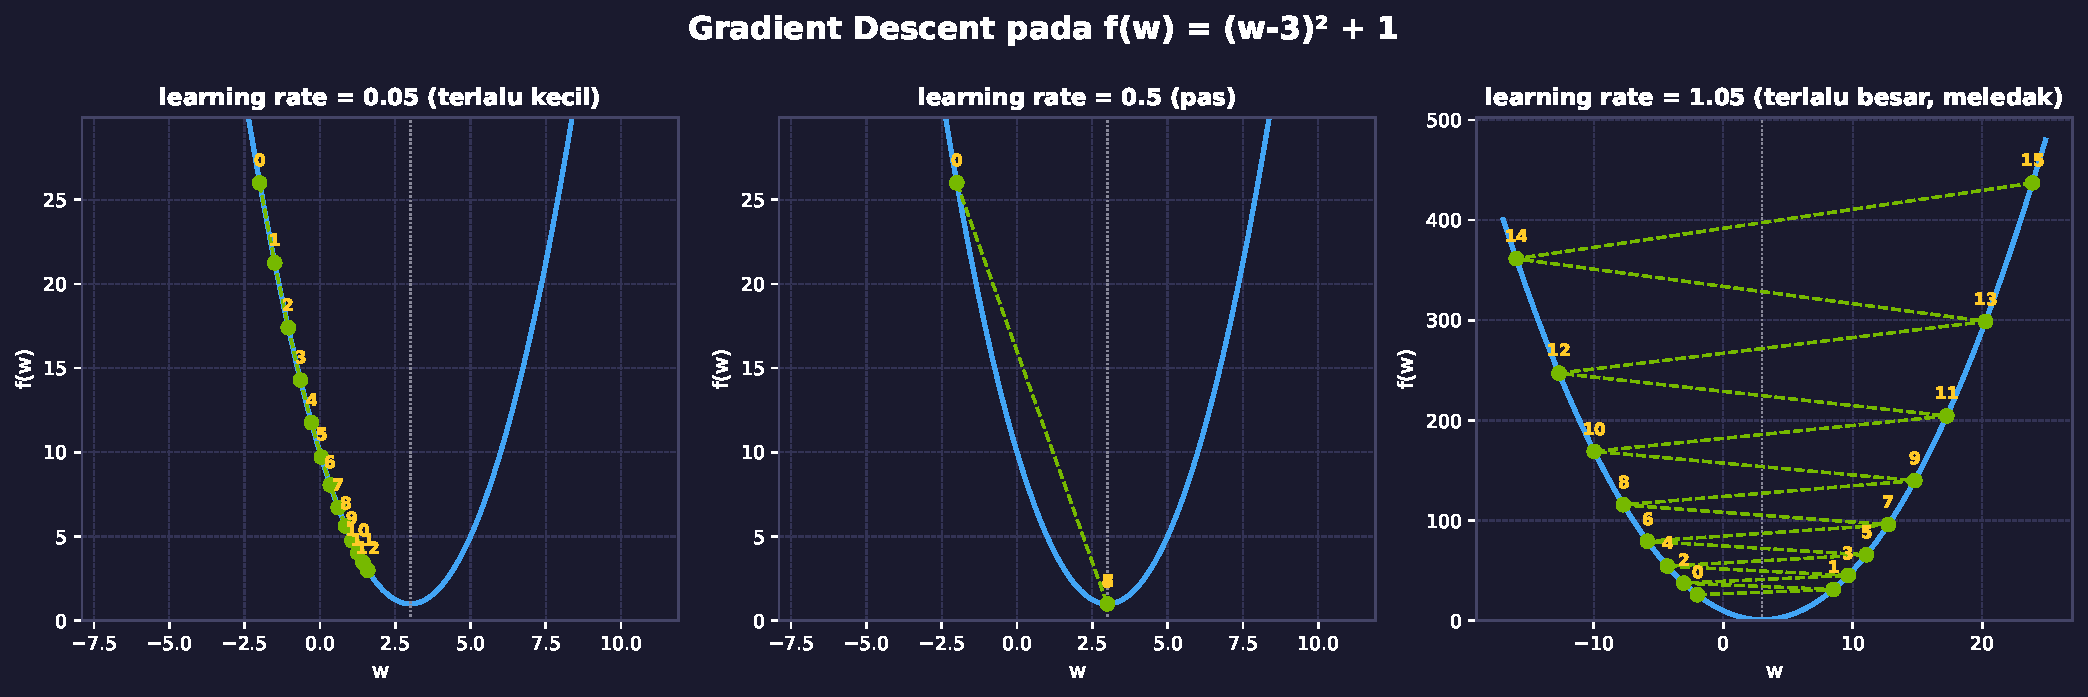
\includegraphics[width=0.96\textwidth, height=3.4cm, keepaspectratio]{figures/gradient_descent.pdf}
  \end{center}
  \vspace{0.1em}
  \nvbox{Intinya}{Bentuk seluruh bukitnya tidak diketahui. Yang bisa diukur hanya kemiringan
  di titik sekarang; satu langkah diambil ke arah menurun, lalu diulang sampai kemiringannya
  mendekati nol.\\[0.3em]{\footnotesize\color{nvgray}Ketiga panel: fungsi sama, ukuran langkah berbeda.}}
\end{frame}

% ----------------------------------------------------------
% FRAME 10 — Learning rate
% ----------------------------------------------------------
\begin{frame}{Learning rate: ukuran langkah dan gejalanya}
  \vspace{0.3em}
  \begin{columns}[T]
    \begin{column}{0.48\textwidth}
      \textbf{\color{nvlightgreen}Terlalu kecil}
      \vspace{0.35em}
      \begin{itemize}\setlength\itemsep{0.38em}
        \item Loss turun, tetapi sangat lambat
        \item Panel kiri: 12 langkah belum sampai ke dasar
        \item Epoch habis sebelum modelnya selesai belajar
      \end{itemize}
    \end{column}
    \begin{column}{0.48\textwidth}
      \textbf{\color{nvred}Terlalu besar}
      \vspace{0.35em}
      \begin{itemize}\setlength\itemsep{0.38em}
        \item Langkahnya melewati dasar, lalu menjauh
        \item Panel kanan: nilai $w$ makin jauh tiap langkah
        \item Loss naik-turun tanpa arah, atau menjadi NaN
      \end{itemize}
    \end{column}
  \end{columns}
  \vspace{0.9em}
  \jebakan{Adam memakai learning rate 0,001 sebagai nilai default. Itu titik awal yang
  wajar, bukan angka yang cocok untuk semua data. Kalau loss diam saja atau meledak sejak
  epoch pertama, ubah dulu learning ratenya sebelum menambah layer.}
\end{frame}

% ----------------------------------------------------------
% FRAME 11 — Intuisi: backprop
% ----------------------------------------------------------
\begin{frame}
  \intuisi{Backprop: kesalahan dibagi ke belakang}
  \vspace{0.4em}
  \begin{center}
  \begin{tikzpicture}[font=\scriptsize,
    lay/.style={fill=nvcard, rounded corners=4pt, text=nvwhite, inner sep=6pt,
                minimum height=0.95cm, minimum width=1.85cm, align=center}]
    \node[lay] (i)  at (0,0)    {input};
    \node[lay] (h1) at (2.85,0) {hidden 1};
    \node[lay] (h2) at (5.7,0)  {hidden 2};
    \node[lay] (o)  at (8.55,0) {keluaran};
    \node[fill=nvorange!30!nvbg, draw=nvorange, rounded corners=4pt, text=nvwhite,
          inner sep=5pt] (l) at (11.1,0) {loss};
    \draw[nvgreen, line width=1pt, -{Stealth[length=5pt]}] (i) -- (h1);
    \draw[nvgreen, line width=1pt, -{Stealth[length=5pt]}] (h1) -- (h2);
    \draw[nvgreen, line width=1pt, -{Stealth[length=5pt]}] (h2) -- (o);
    \draw[nvgreen, line width=1pt, -{Stealth[length=5pt]}] (o) -- (l);
    \node[text=nvgreen, anchor=south] at (5.7,0.62) {maju: hitung prediksi};
    \draw[nvorange, line width=1pt, -{Stealth[length=5pt]}] (11.1,-1.1) -- (8.55,-1.1);
    \draw[nvorange, line width=1pt, -{Stealth[length=5pt]}] (8.55,-1.1) -- (5.7,-1.1);
    \draw[nvorange, line width=1pt, -{Stealth[length=5pt]}] (5.7,-1.1) -- (2.85,-1.1);
    \draw[nvorange, line width=1pt, -{Stealth[length=5pt]}] (2.85,-1.1) -- (0,-1.1);
    \node[text=nvorange, anchor=north] at (5.7,-1.35) {mundur: bagi kesalahan ke tiap bobot};
  \end{tikzpicture}
  \end{center}
  \vspace{0.4em}
  \nvbox{Intinya}{Setelah loss dihitung di keluaran, tiap bobot menerima satu angka:
  seberapa besar sumbangannya terhadap kesalahan itu. Bobot yang menyumbang lebih banyak
  digeser lebih jauh.}
\end{frame}

% ----------------------------------------------------------
% FRAME 12 — Epoch dan batch
% ----------------------------------------------------------
\begin{frame}{Epoch, batch, dan satu langkah perbaikan}
  \vspace{0.3em}
  \begin{center}
  \begin{tikzpicture}[font=\scriptsize,
    b/.style={fill=nvcard, rounded corners=3pt, text=nvwhite, inner sep=4pt,
              minimum width=1.35cm, minimum height=0.62cm}]
    \node[text=nvgray, anchor=east] at (-0.35,0) {1 epoch};
    \node[b] (b1) at (0.8,0) {batch 1};
    \node[b] (b2) at (2.45,0) {batch 2};
    \node[b] (b3) at (4.1,0) {batch 3};
    \node[text=nvgray] at (5.5,0) {\dots};
    \node[b] (b4) at (7.4,0) {batch 1.718};
    \foreach \n in {b1,b2,b3,b4}
      \draw[nvgreen, -{Stealth[length=4pt]}] (\n.south) -- ++(0,-0.5);
    \node[text=nvgreen, anchor=north, align=center] at (0.8,-0.9) {bobot\\ diperbarui};
    \node[text=nvgreen, anchor=north, align=center] at (2.45,-0.9) {bobot\\ diperbarui};
    \node[text=nvgreen, anchor=north, align=center] at (4.1,-0.9) {bobot\\ diperbarui};
    \node[text=nvgreen, anchor=north, align=center] at (7.4,-0.9) {bobot\\ diperbarui};
    \draw[nvgray, -{Stealth[length=4pt]}] (8.55,0) -- (9.75,0)
      node[right, text=nvwhite, align=left] {epoch\\ berikutnya};
  \end{tikzpicture}
  \end{center}
  \vspace{0.5em}
  \begin{itemize}\setlength\itemsep{0.34em}
    \item Satu batch berisi 32 gambar yang dihitung bersama. Bobot diperbarui sekali
          untuk setiap batch.
    \item Satu epoch berarti seluruh data train dilewati sekali: 55.000 gambar dibagi 32
          memberi 1.718 langkah perbaikan.
    \item Batch lebih besar membuat arah langkahnya lebih tenang, tetapi butuh memori
          lebih besar dan langkahnya lebih sedikit per epoch.
  \end{itemize}
  \vspace{0.3em}
  {\footnotesize\color{nvgray}Angka ini dari nb01: 55.000 data train, 5.000 validation,
  10.000 test.}
\end{frame}

% ----------------------------------------------------------
% FRAME 13 — Kurva train vs validation
% ----------------------------------------------------------
\begin{frame}{Kurva train dan validation dibaca berdampingan}
  \vspace{0.1em}
  \begin{center}
    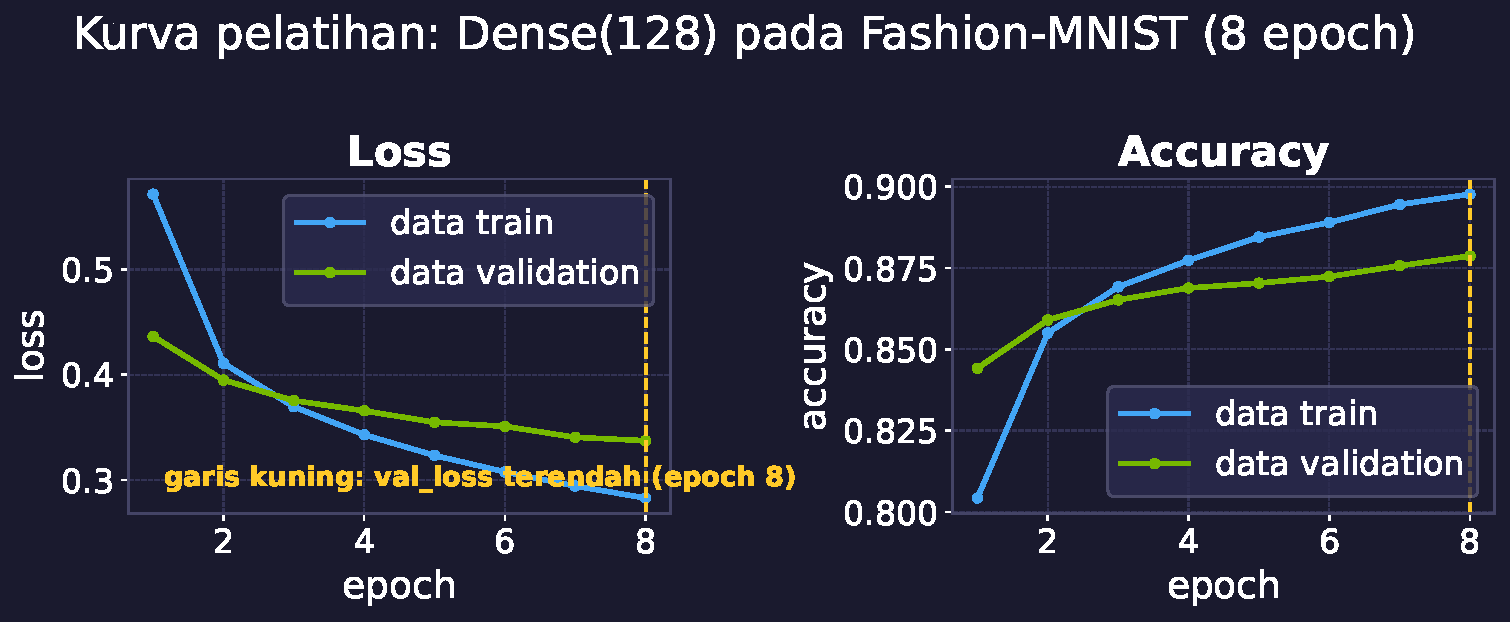
\includegraphics[width=0.84\textwidth, height=3.4cm, keepaspectratio]{figures/train_curves.pdf}
  \end{center}
  \vspace{0.1em}
  \begin{itemize}\setlength\itemsep{0.3em}
    \item Kedua kurva loss masih turun bersama, dan akurasi validation berhenti di
          sekitar 0,88.
    \item Kalau loss validation mulai naik sementara loss train terus turun, model mulai
          menghafal data train.
    \item Pada run ini val\_loss terendah jatuh di epoch terakhir, jadi 8 epoch belum
          cukup untuk melihat titik baliknya.
  \end{itemize}
\end{frame}

% ----------------------------------------------------------
% FRAME 14 — Overfitting: dropout dan early stopping
% ----------------------------------------------------------
\begin{frame}{Overfitting: melebarnya jarak train dan validation}
  \begin{center}
    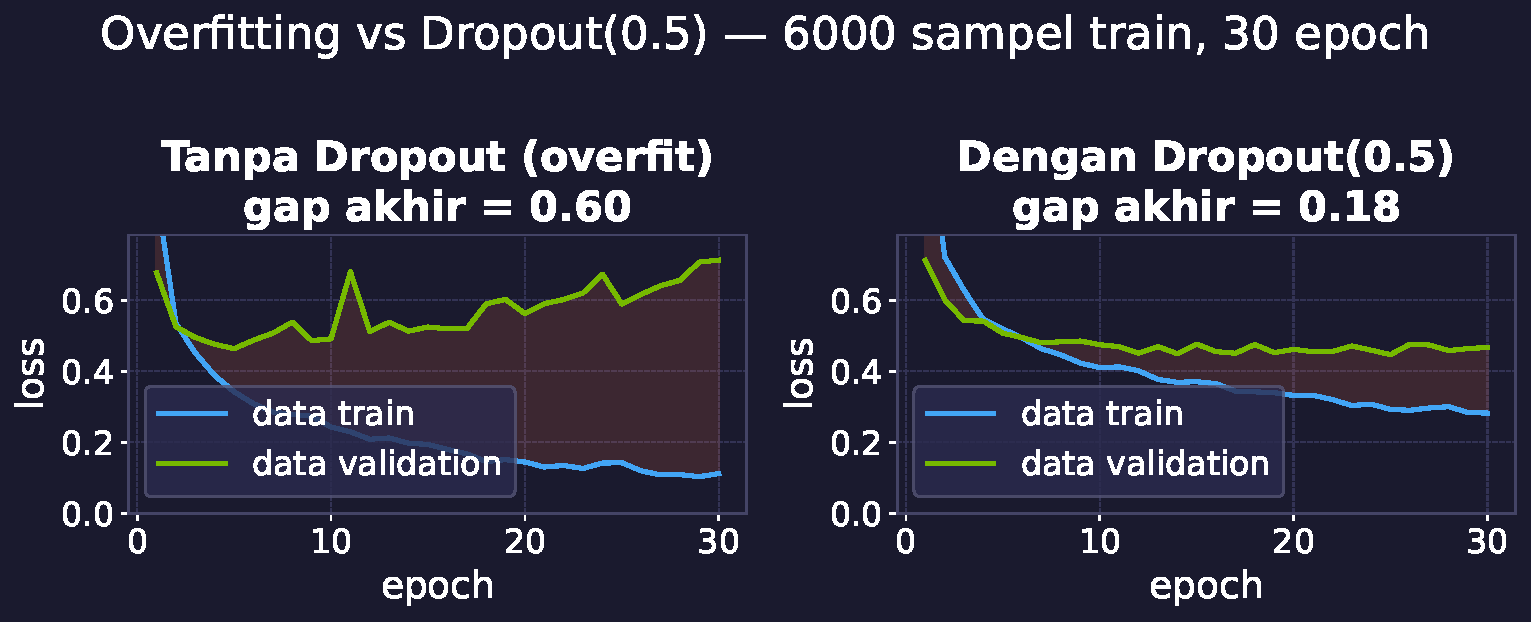
\includegraphics[width=0.64\textwidth, height=2.8cm, keepaspectratio]{figures/overfit_curves.pdf}
  \end{center}
  \begin{itemize}\setlength\itemsep{0.24em}
    \item Model yang sama pada 6.000 sampel train: jaraknya 0,56 tanpa dropout dan 0,18
          dengan Dropout(0,5).
    \item Dropout mematikan sebagian neuron secara acak tiap batch; early stopping
          berhenti saat val\_loss tidak lagi turun.
  \end{itemize}
  \jebakan{Dropout hanya aktif saat training. Loss validation yang lebih rendah daripada
  loss train bukan keajaiban: saat evaluasi, dropoutnya dimatikan.}
\end{frame}

% ----------------------------------------------------------
% FRAME 15 — Normalisasi input
% ----------------------------------------------------------
\begin{frame}{Normalisasi input: dari 0--255 ke 0,0--1,0}
  \vspace{0.4em}
  \begin{center}
  \begin{tikzpicture}[font=\scriptsize]
    \shade[left color=nvbg, right color=nvwhite, draw=nvgray]
      (0,1.1) rectangle (7.5,1.75);
    \node[text=nvwhite, anchor=east] at (-0.3,1.42) {nilai pixel};
    \node[text=nvgray, anchor=north] at (0,1.05) {0};
    \node[text=nvgray, anchor=north] at (7.5,1.05) {255};
    \shade[left color=nvbg, right color=nvlightgreen, draw=nvgray]
      (0,-0.35) rectangle (7.5,0.3);
    \node[text=nvwhite, anchor=east] at (-0.3,-0.02) {setelah dibagi 255};
    \node[text=nvgray, anchor=north] at (0,-0.4) {0,0};
    \node[text=nvgray, anchor=north] at (7.5,-0.4) {1,0};
    \draw[nvgreen, line width=1pt, -{Stealth[length=5pt]}] (8.2,1.42)
      .. controls (9.3,1.42) and (9.3,-0.02) .. (8.2,-0.02);
    \node[text=nvgreen, anchor=west] at (9.5,0.7) {dibagi 255};
  \end{tikzpicture}
  \end{center}
  \vspace{0.6em}
  \begin{itemize}\setlength\itemsep{0.34em}
    \item Masukan dengan rentang besar membuat gradientnya besar juga, sehingga langkah
          gradient descent sulit diatur dengan satu learning rate.
    \item Untuk pixel, pembaginya konstanta 255. Untuk data tabular, statistik scalingnya
          dihitung dari data train saja, lalu dipakai apa adanya ke validation dan test.
  \end{itemize}
\end{frame}

% ----------------------------------------------------------
% FRAME 16 — Evaluasi multi-kelas
% ----------------------------------------------------------
\begin{frame}{Evaluasi multi-kelas: akurasi saja belum cukup}
  \vspace{0.2em}
  \begin{columns}[T]
    \begin{column}{0.44\textwidth}
      \begin{center}
        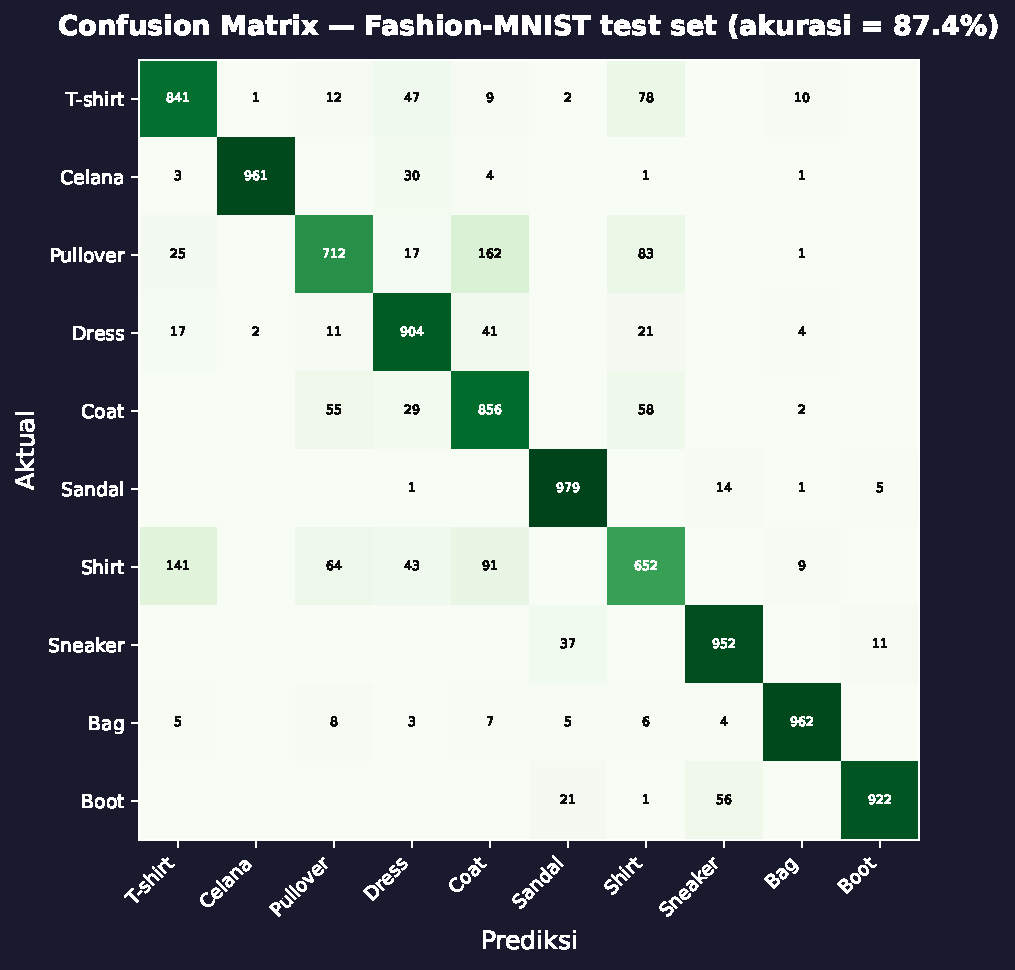
\includegraphics[width=\textwidth, height=4.65cm, keepaspectratio]{figures/confusion.pdf}
      \end{center}
    \end{column}
    \begin{column}{0.54\textwidth}
      \vspace{0.3em}
      \begin{itemize}\setlength\itemsep{0.42em}
        \item Akurasi test 87,4\% pada model Dense(128) di gambar ini: satu run, seed 42,
              data test disentuh sekali.
        \item Diagonal berisi prediksi yang benar. Sel di luar diagonal menunjukkan kelas
              apa tertukar dengan apa.
        \item Pasangan yang paling sering tertukar dihitung dari matriksnya, dan bisa
              berbeda tiap kali model dilatih ulang.
        \item Kelas dengan bentuk khas lebih jarang tertukar daripada kelas yang
              potongannya mirip.
      \end{itemize}
    \end{column}
  \end{columns}
\end{frame}

% ----------------------------------------------------------
% FRAME 17 — Ringkasan Act 1
% ----------------------------------------------------------
\begin{frame}{Ringkasan Act 1}
  \vspace{0.5em}
  \begin{itemize}\setlength\itemsep{0.46em}
    \item Satu neuron menghitung jumlah berbobot dari masukannya, menambah bias, lalu
          melewatkannya ke aktivasi. Layer adalah kumpulan neuron seperti itu.
    \item Loss meringkas kesalahan menjadi satu angka. Gradient descent menurunkannya
          dengan langkah kecil ke arah menurun, dan backprop membagi kesalahan itu ke
          tiap bobot.
    \item Learning rate menentukan ukuran langkah: terlalu kecil membuat training lambat,
          terlalu besar membuatnya meledak.
    \item Kurva train dan validation dibaca bersama. Jarak yang melebar adalah tanda
          overfitting, dan dropout serta early stopping menahannya.
    \item Untuk klasifikasi banyak kelas, confusion matrix menunjukkan kesalahan yang
          tidak terlihat dari angka akurasi.
  \end{itemize}
\end{frame}

% ==========================================================
% ACT 2
% ==========================================================
\acttitle{Act 2}{\fontsize{28}{32}\selectfont\bfseries Kenapa butuh aktivasi?}{Tanpa aktivasi, seratus layer sama saja dengan satu layer}

% ----------------------------------------------------------
% FRAME 19 — Tanpa aktivasi tetap linear
% ----------------------------------------------------------
\begin{frame}{Tanpa aktivasi, tumpukan layer tetap satu garis}
  \vspace{0.4em}
  \begin{center}
  \begin{tikzpicture}[font=\scriptsize,
    lay/.style={fill=nvcard, rounded corners=4pt, text=nvwhite, inner sep=6pt,
                minimum height=0.9cm, minimum width=1.5cm}]
    \node[lay] (l1) at (0,0)    {$W_1, b_1$};
    \node[lay] (l2) at (2.1,0)  {$W_2, b_2$};
    \node[lay] (l3) at (4.2,0)  {$W_3, b_3$};
    \draw[nvgreen, -{Stealth[length=4pt]}] (l1) -- (l2);
    \draw[nvgreen, -{Stealth[length=4pt]}] (l2) -- (l3);
    \node[text=nvorange, font=\Large] at (5.75,0) {$=$};
    \node[lay, draw=nvorange] (one) at (7.5,0) {$W, b$};
    \node[text=nvgray, anchor=north, align=center] at (2.1,-0.7)
      {tiga layer linear ditumpuk};
    \node[text=nvgray, anchor=north, align=center] at (7.5,-0.7)
      {satu layer linear};
  \end{tikzpicture}
  \end{center}
  \vspace{0.5em}
  \begin{center}
    \color{nvlightgreen}$W_2\left(W_1x + b_1\right) + b_2 = \left(W_2W_1\right)x + \left(W_2b_1 + b_2\right)$
  \end{center}
  \vspace{0.5em}
  \begin{itemize}\setlength\itemsep{0.32em}
    \item Hasil dua layer linear bisa ditulis ulang sebagai satu layer linear,
          jadi menambah layer tidak menambah bentuk yang bisa dipelajari.
    \item nb02 memakai model tanpa aktivasi sebagai baseline linear, lalu membandingkannya
          dengan model yang beraktivasi.
  \end{itemize}
\end{frame}

% ----------------------------------------------------------
% FRAME 20 — Empat aktivasi dan turunannya
% ----------------------------------------------------------
\begin{frame}{Empat aktivasi dan turunannya}
  \vspace{0.1em}
  \begin{center}
    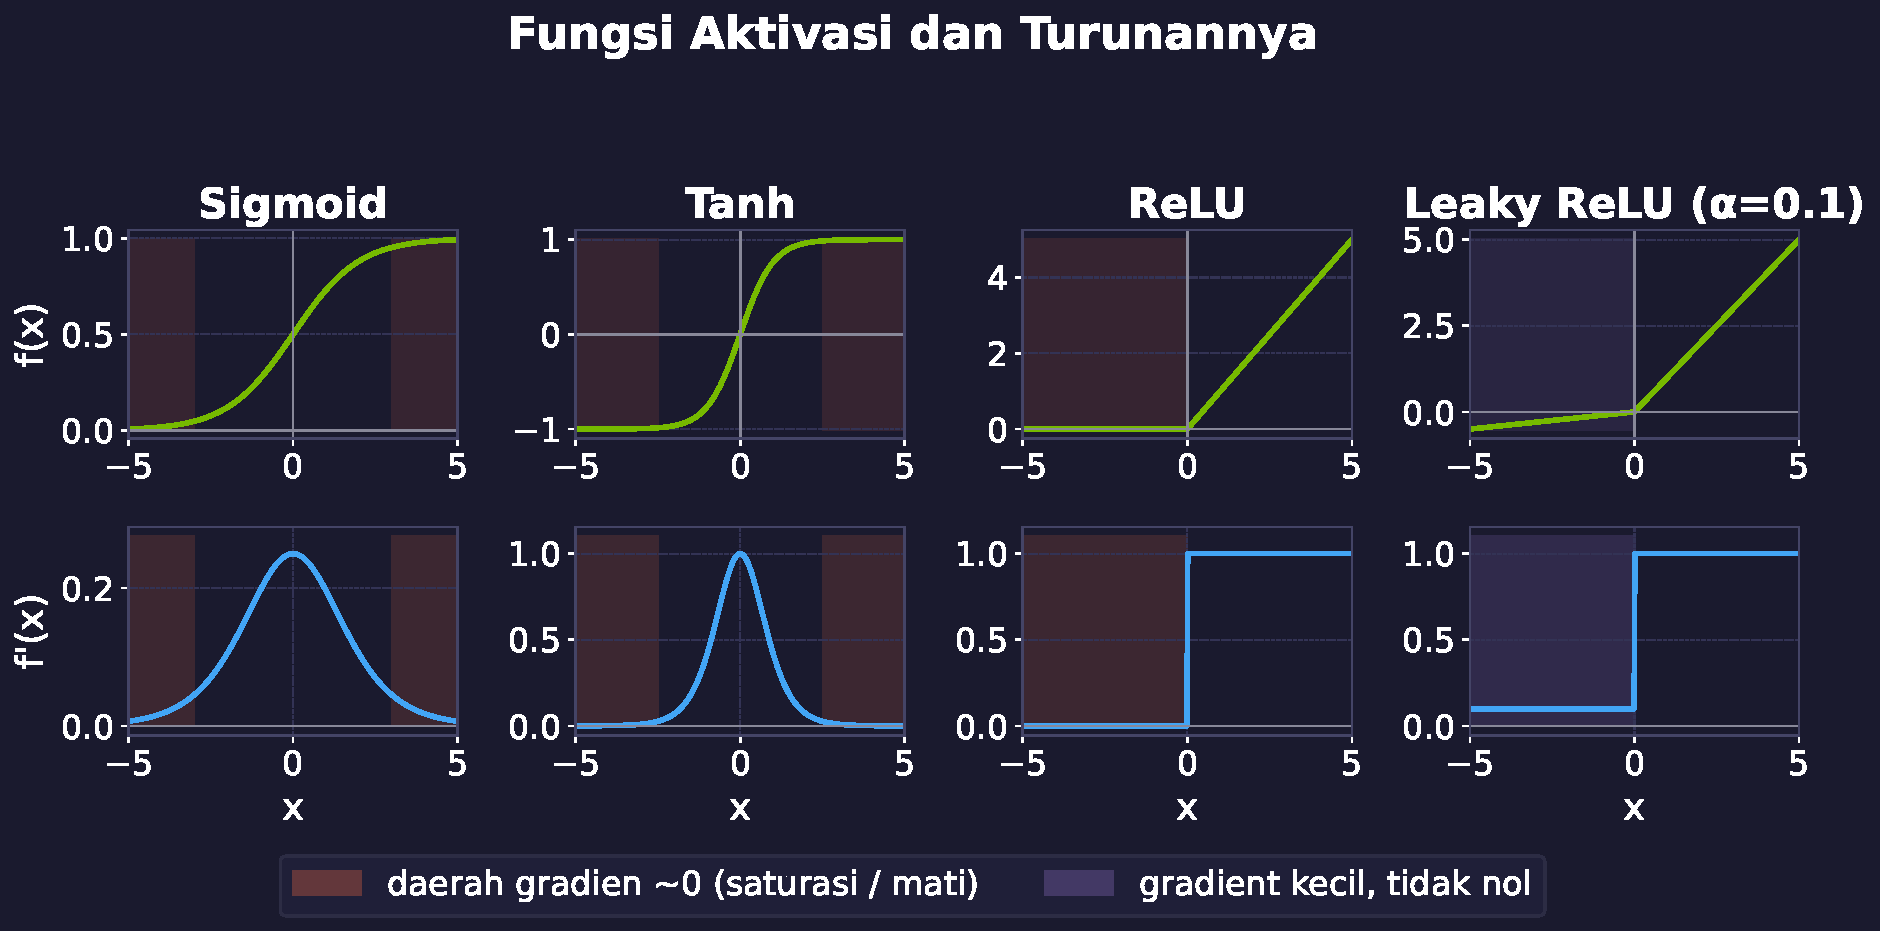
\includegraphics[width=0.94\textwidth, height=4.5cm, keepaspectratio]{figures/activations.pdf}
  \end{center}
  \vspace{0.15em}
  \begin{itemize}\setlength\itemsep{0.28em}
    \item Baris atas fungsinya, baris bawah turunannya. Turunan inilah yang dipakai backprop.
    \item Daerah merah menandai tempat turunannya mendekati nol; bobot di sana hampir tidak
          berubah.
  \end{itemize}
\end{frame}

% ----------------------------------------------------------
% FRAME 21 — Intuisi: vanishing gradient
% ----------------------------------------------------------
\begin{frame}
  \intuisi{Vanishing gradient: pesan yang habis di jalan}
  \vspace{0.5em}
  \begin{center}
  \begin{tikzpicture}[font=\scriptsize,
    lay/.style={fill=nvcard, rounded corners=4pt, text=nvwhite, inner sep=6pt,
                minimum height=0.9cm, minimum width=1.7cm}]
    \node[lay] (l1) at (0,0)   {layer 1};
    \node[lay] (l2) at (2.9,0) {layer 2};
    \node[lay] (l3) at (5.8,0) {layer 3};
    \node[lay] (l4) at (8.7,0) {layer 4};
    \node[fill=nvorange!30!nvbg, draw=nvorange, rounded corners=4pt, text=nvwhite,
          inner sep=5pt] (ls) at (11.2,0) {loss};
    \draw[nvorange, line width=1pt, -{Stealth[length=5pt]}] (ls) -- (l4)
      node[midway, above, text=nvorange, font=\tiny] {1};
    \draw[nvorange, line width=1pt, -{Stealth[length=5pt]}] (l4) -- (l3)
      node[midway, above, text=nvorange, font=\tiny] {$\times$ 0,25};
    \draw[nvorange, line width=1pt, -{Stealth[length=5pt]}] (l3) -- (l2)
      node[midway, above, text=nvorange, font=\tiny] {$\times$ 0,25};
    \draw[nvorange, line width=1pt, -{Stealth[length=5pt]}] (l2) -- (l1)
      node[midway, above, text=nvorange, font=\tiny] {$\times$ 0,25};
    \node[text=nvgray, anchor=north] at (1.45,-0.65) {yang sampai ke layer 1: sekitar 0,016};
  \end{tikzpicture}
  \end{center}
  \vspace{0.5em}
  \nvbox{Intinya}{Turunan sigmoid paling besar 0,25. Saat kesalahan dibagi ke belakang
  melewati banyak layer, angkanya dikalikan berulang dan mengecil cepat, sehingga layer
  paling awal hampir tidak ikut belajar.}
\end{frame}

% ----------------------------------------------------------
% FRAME 22 — ReLU dan Leaky ReLU
% ----------------------------------------------------------
\begin{frame}{ReLU: turunannya tetap 1 di sisi positif}
  \vspace{0.2em}
  \begin{columns}[T]
    \begin{column}{0.34\textwidth}
      \centering
      \textbf{\color{nvgreen}ReLU}\\[0.3em]
      \begin{tikzpicture}[scale=0.78, font=\tiny]
        \draw[nvgray, ->] (-1.7,0) -- (1.9,0) node[below left, text=nvgray] {$x$};
        \draw[nvgray, ->] (0,-0.7) -- (0,1.9) node[left, text=nvgray] {$f(x)$};
        \draw[nvgreen, line width=1.3pt] (-1.6,0) -- (0,0) -- (1.7,1.7);
      \end{tikzpicture}\\[0.3em]
      {\scriptsize $f(x)=\max(0,\,x)$}\\[0.5em]
      \textbf{\color{nvlightgreen}Leaky ReLU}\\[0.3em]
      \begin{tikzpicture}[scale=0.78, font=\tiny]
        \draw[nvgray, ->] (-1.7,0) -- (1.9,0) node[below left, text=nvgray] {$x$};
        \draw[nvgray, ->] (0,-0.7) -- (0,1.9) node[left, text=nvgray] {$f(x)$};
        \draw[nvlightgreen, line width=1.3pt] (-1.6,-0.16) -- (0,0) -- (1.7,1.7);
      \end{tikzpicture}
    \end{column}
    \begin{column}{0.62\textwidth}
      \vspace{0.2em}
      \begin{itemize}\setlength\itemsep{0.35em}
        \item ReLU meneruskan nilai positif apa adanya dan menolkan yang negatif.
              Turunannya 1 di sisi positif, jadi kesalahan tidak menyusut saat dibagi
              ke belakang.
        \item Perhitungannya juga murah: satu perbandingan dengan nol per neuron.
        \item Sisi negatifnya nol. Neuron yang masukannya negatif terus berhenti
              diperbarui, dan keadaan itu disebut dead ReLU.
        \item Leaky ReLU memberi kemiringan kecil di sisi negatif, 0,1 pada gambar
              sebelumnya, sehingga masih ada gradient yang mengalir.
      \end{itemize}
    \end{column}
  \end{columns}
\end{frame}

% ----------------------------------------------------------
% FRAME 23 — Softmax
% ----------------------------------------------------------
\begin{frame}{Softmax: skor mentah menjadi probabilitas}
  \vspace{0.2em}
  \begin{center}
    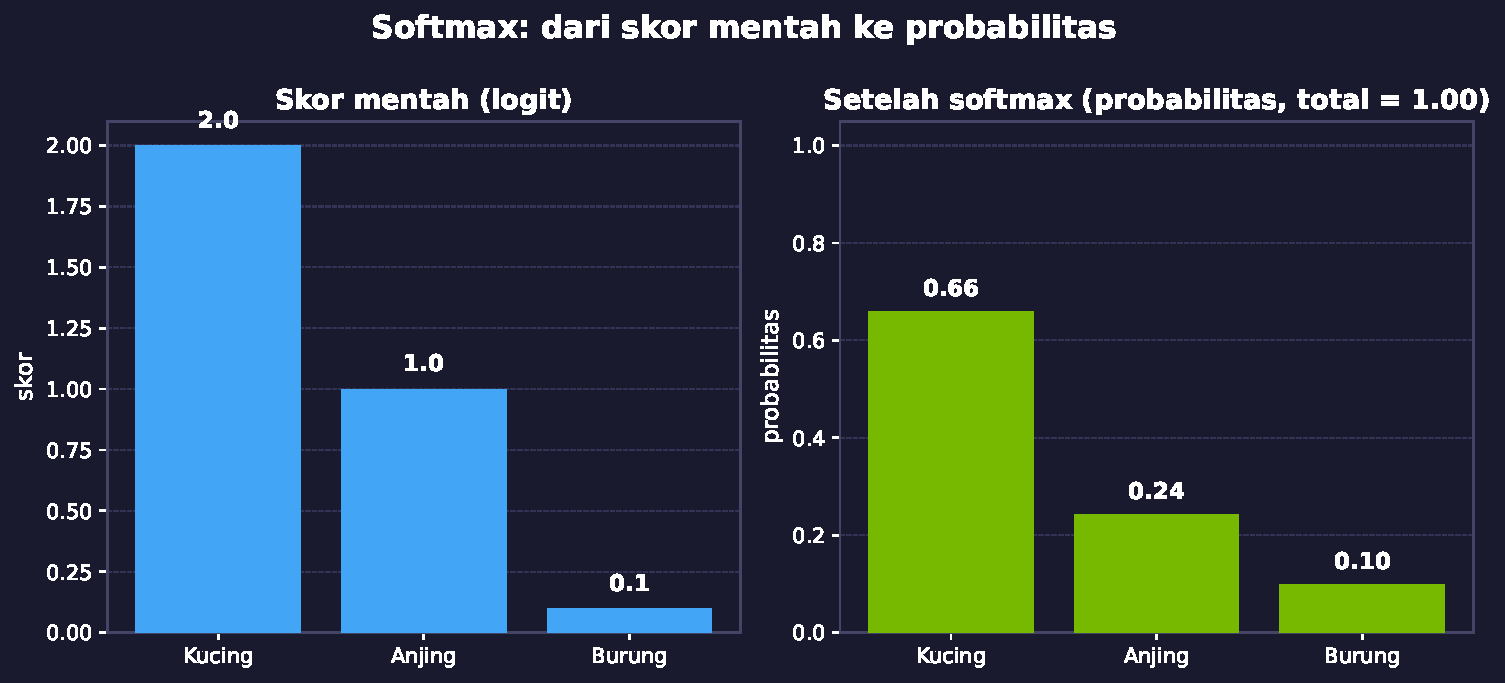
\includegraphics[width=0.63\textwidth, height=3.25cm, keepaspectratio]{figures/softmax.pdf}
  \end{center}
  \vspace{0.3em}
  \begin{itemize}\setlength\itemsep{0.34em}
    \item Softmax bekerja pada seluruh output layer sekaligus: skor 2,0; 1,0; dan 0,1
          menjadi 0,66; 0,24; dan 0,10, dengan total tepat 1.
    \item Selisih skor satu poin menjadi selisih probabilitas yang cukup besar, karena
          skornya lewat fungsi eksponensial dulu.
    \item Untuk dua kelas, satu keluaran dengan sigmoid sudah cukup. Untuk regresi, output
          layer dibiarkan tanpa aktivasi.
  \end{itemize}
\end{frame}

% ----------------------------------------------------------
% FRAME 24 — Intuisi: optimizer
% ----------------------------------------------------------
\begin{frame}
  \intuisi{Optimizer: cara berbeda menuruni bukit yang sama}
  \vspace{0.3em}
  \begin{center}
  \begin{tikzpicture}[font=\scriptsize]
    \foreach \r in {0.45,0.8,1.15,1.5}
      \draw[nvgray!55!nvbg, line width=0.8pt] (0,0) ellipse ({\r*2.1} and {\r*1.05});
    \fill[nvwhite] (0,0) circle (1.8pt);
    \node[text=nvgray, anchor=west, font=\tiny] at (0.16,0.02) {minimum};
    \draw[nvred, line width=1pt]
      (-2.85,1.15) -- (-2.05,-0.35) -- (-1.35,0.7) -- (-0.7,-0.3) -- (-0.25,0.25) -- (0,0);
    \draw[nvorange, line width=1pt]
      (-2.85,1.15) -- (-1.75,0.05) -- (-0.9,0.3) -- (-0.28,-0.08) -- (0,0);
    \draw[nvgreen, line width=1.3pt]
      (-2.85,1.15) .. controls (-1.6,0.5) and (-0.7,0.1) .. (0,0);
    \node[text=nvred, anchor=west] at (3.45,1.1) {SGD};
    \node[text=nvorange, anchor=west] at (3.45,0.65) {SGD + momentum};
    \node[text=nvgreen, anchor=west] at (3.45,0.2) {Adam};
    \node[text=nvgray, anchor=west, font=\tiny, align=left] at (3.45,-0.55)
      {garis oval = tempat\\ dengan loss sama};
  \end{tikzpicture}
  \end{center}
  \vspace{0.3em}
  \nvbox{Intinya}{SGD melangkah menurut kemiringan saat itu saja. Momentum menambahkan
  sisa arah langkah sebelumnya, sehingga jalurnya tidak banyak berbelok. Adam menyimpan
  rata-rata arah dan besar gradient, lalu menyesuaikan ukuran langkah tiap parameter.}
\end{frame}

% ----------------------------------------------------------
% FRAME 25 — Kapan mengganti default & jebakan
% ----------------------------------------------------------
\begin{frame}{Kapan mengganti aktivasi atau optimizer default}
  \vspace{0.3em}
  \kapan{
    \item banyak neuron ReLU berhenti aktif, keluarannya nol terus
    \item loss diam sejak epoch awal padahal datanya sudah dinormalisasi
    \item jaringannya dalam dan layer awalnya hampir tidak berubah
  }{
    \item lossnya belum turun karena learning ratenya belum disesuaikan
    \item perbandingannya belum diuji di data validation
    \item modelnya masih underfit dan layernya memang terlalu sedikit
  }
  \vspace{0.7em}
  \jebakan{Dead ReLU biasanya berawal dari learning rate yang terlalu besar, bukan dari
  ReLU itu sendiri. Kalau lossnya tidak turun, ganti learning ratenya dulu, sebelum
  arsitekturnya.}
\end{frame}

% ----------------------------------------------------------
% FRAME 26 — Ringkasan Act 2
% ----------------------------------------------------------
\begin{frame}{Ringkasan Act 2}
  \vspace{0.5em}
  \begin{itemize}\setlength\itemsep{0.46em}
    \item Aktivasi adalah bagian yang membuat tumpukan layer bisa mempelajari pola
          melengkung. Tanpa aktivasi, hasil akhirnya tetap satu layer linear.
    \item Sigmoid dan tanh punya turunan yang mengecil di kedua ujung, sehingga kesalahan
          menyusut saat dibagi ke belakang melewati banyak layer.
    \item ReLU menjaga turunannya tetap 1 di sisi positif dan murah dihitung, jadi dipakai
          sebagai pilihan awal untuk hidden layer. Leaky ReLU menyisakan gradient kecil di
          sisi negatif.
    \item Softmax dipakai di output layer klasifikasi banyak kelas; sigmoid untuk dua
          kelas; tanpa aktivasi untuk regresi.
    \item Optimizer hanya mengubah cara melangkah, bukan bukitnya. Adam menjadi titik
          awal yang wajar, dan learning ratenya tetap perlu diperiksa.
  \end{itemize}
\end{frame}

\end{document}
